\subsection{\texorpdfstring{\ttbar}{ttbar} Irreducible Background
\label{sec:ttbarbkg}}

% Special symbols for ttbar estimation
\newcommand{\Be}{\ensuremath{\mathcal{B}_{\W\Pe}}\xspace}
\newcommand{\Bm}{\ensuremath{\mathcal{B}_{\W\mu}}\xspace}
\newcommand{\Bl}{\ensuremath{\mathcal{B}_{\W\ell}}\xspace}
\newcommand{\Bte}{\ensuremath{\mathcal{B}_{\W\tau_{\Pe}}}\xspace}
\newcommand{\Btm}{\ensuremath{\mathcal{B}_{\W\tau_{\mu}}}\xspace}
\newcommand{\Btl}{\ensuremath{\mathcal{B}_{\W\tau_{\ell}}}\xspace}
\newcommand{\Bth}{\ensuremath{\mathcal{B}_{\W\tauh}}\xspace}
\newcommand{\Aem}{\ensuremath{\mathcal{A}_{\Pe\mu}}\xspace}
\newcommand{\Amte}{\ensuremath{\mathcal{A}_{\mu\tau_{\Pe}}}\xspace}
\newcommand{\Amtm}{\ensuremath{\mathcal{A}_{\mu\tau_{\mu}}}\xspace}
\newcommand{\Amtl}{\ensuremath{\mathcal{A}_{\mu\tau_{\ell}}}\xspace}
\newcommand{\Amth}{\ensuremath{\mathcal{A}_{\mu\tauh}}\xspace}
\newcommand{\Aete}{\ensuremath{\mathcal{A}_{\Pe\tau_{\Pe}}}\xspace}
\newcommand{\Aeth}{\ensuremath{\mathcal{A}_{\Pe\tauh}}\xspace}
\newcommand{\Aetm}{\ensuremath{\mathcal{A}_{\Pe\tau_{\mu}}}\xspace}
\newcommand{\Aetl}{\ensuremath{\mathcal{A}_{\Pe\tau_{\ell}}}\xspace}
\newcommand{\Alte}{\ensuremath{\mathcal{A}_{\ell\tau_{\Pe}}}\xspace}
\newcommand{\Altm}{\ensuremath{\mathcal{A}_{\ell\tau_{\mu}}}\xspace}
\newcommand{\Altl}{\ensuremath{\mathcal{A}_{\ell\tau_{\ell}}}\xspace}
\newcommand{\Alth}{\ensuremath{\mathcal{A}_{\ell\tauh}}\xspace}
%\newcommand{\Atete}{\ensuremath{\mathcal{A}_{\ell\tau e}}\xspace}
\newcommand{\Atetm}{\ensuremath{\mathcal{A}_{\tau_{\Pe}\tau_{\mu}}}\xspace}
%\newcommand{\Atetl}{\ensuremath{\mathcal{A}_{\ell\tau \ell}}\xspace}
\newcommand{\Atlth}{\ensuremath{\mathcal{A}_{\tau_{\ell}\tauh}}\xspace}
\newcommand{\Ee}{\ensuremath{\varepsilon_{\Pe}^{\text{ID}}}\xspace}
\newcommand{\Emu}{\ensuremath{\varepsilon_{\mu}^{\text{ID}}}\xspace}
\newcommand{\El}{\ensuremath{\varepsilon_{\ell}^{\text{ID}}}\xspace}
\newcommand{\Eth}{\ensuremath{\varepsilon_{\tauh}^{\text{ID}}}\xspace}
\newcommand{\Etl}{\ensuremath{\varepsilon_{\tau_{\ell}}^{\text{ID}}}\xspace}

A large fraction of the background from the \ttbar process is irreducible, due to its similar signature to the signal when both \W bosons produce one muon or electron and one hadronic tau. Thus, the \ttbar irreducible background is one of the dominant backgrounds and has to be estimated precisely. The use of single muon and single electron HLT criteria, along with extra lepton vetoes, enables the definition of a control region of observed events containing one electron and one muon. This \emu control region is used to extrapolate the yield of the \ttbar background in the signal region. It is defined using the selection from the \mutau channel, with the hadronic tau replaced by an electron. For example, the final cut on $\pt(\tauh)$ is applied to the electron in this selection. Figure \ref{fig:ttCC} shows the \ST distributions after the leptoquark final selection in the $\emu$ channel, with good agreement between the observed data and the simulation. The \emu sample consists of approximately 87\% \ttbar events; the residual background from other processes is simulated and subtracted from the observed data. The signal contamination in this sample has been found to be negligible for any signal mass hypothesis. This is expected due to the small branching fraction, only 3\%, for both tau leptons in the signal final state to decay leptonically.

%add more figures here?
\begin{figure}[hbt]
  \begin{center}
    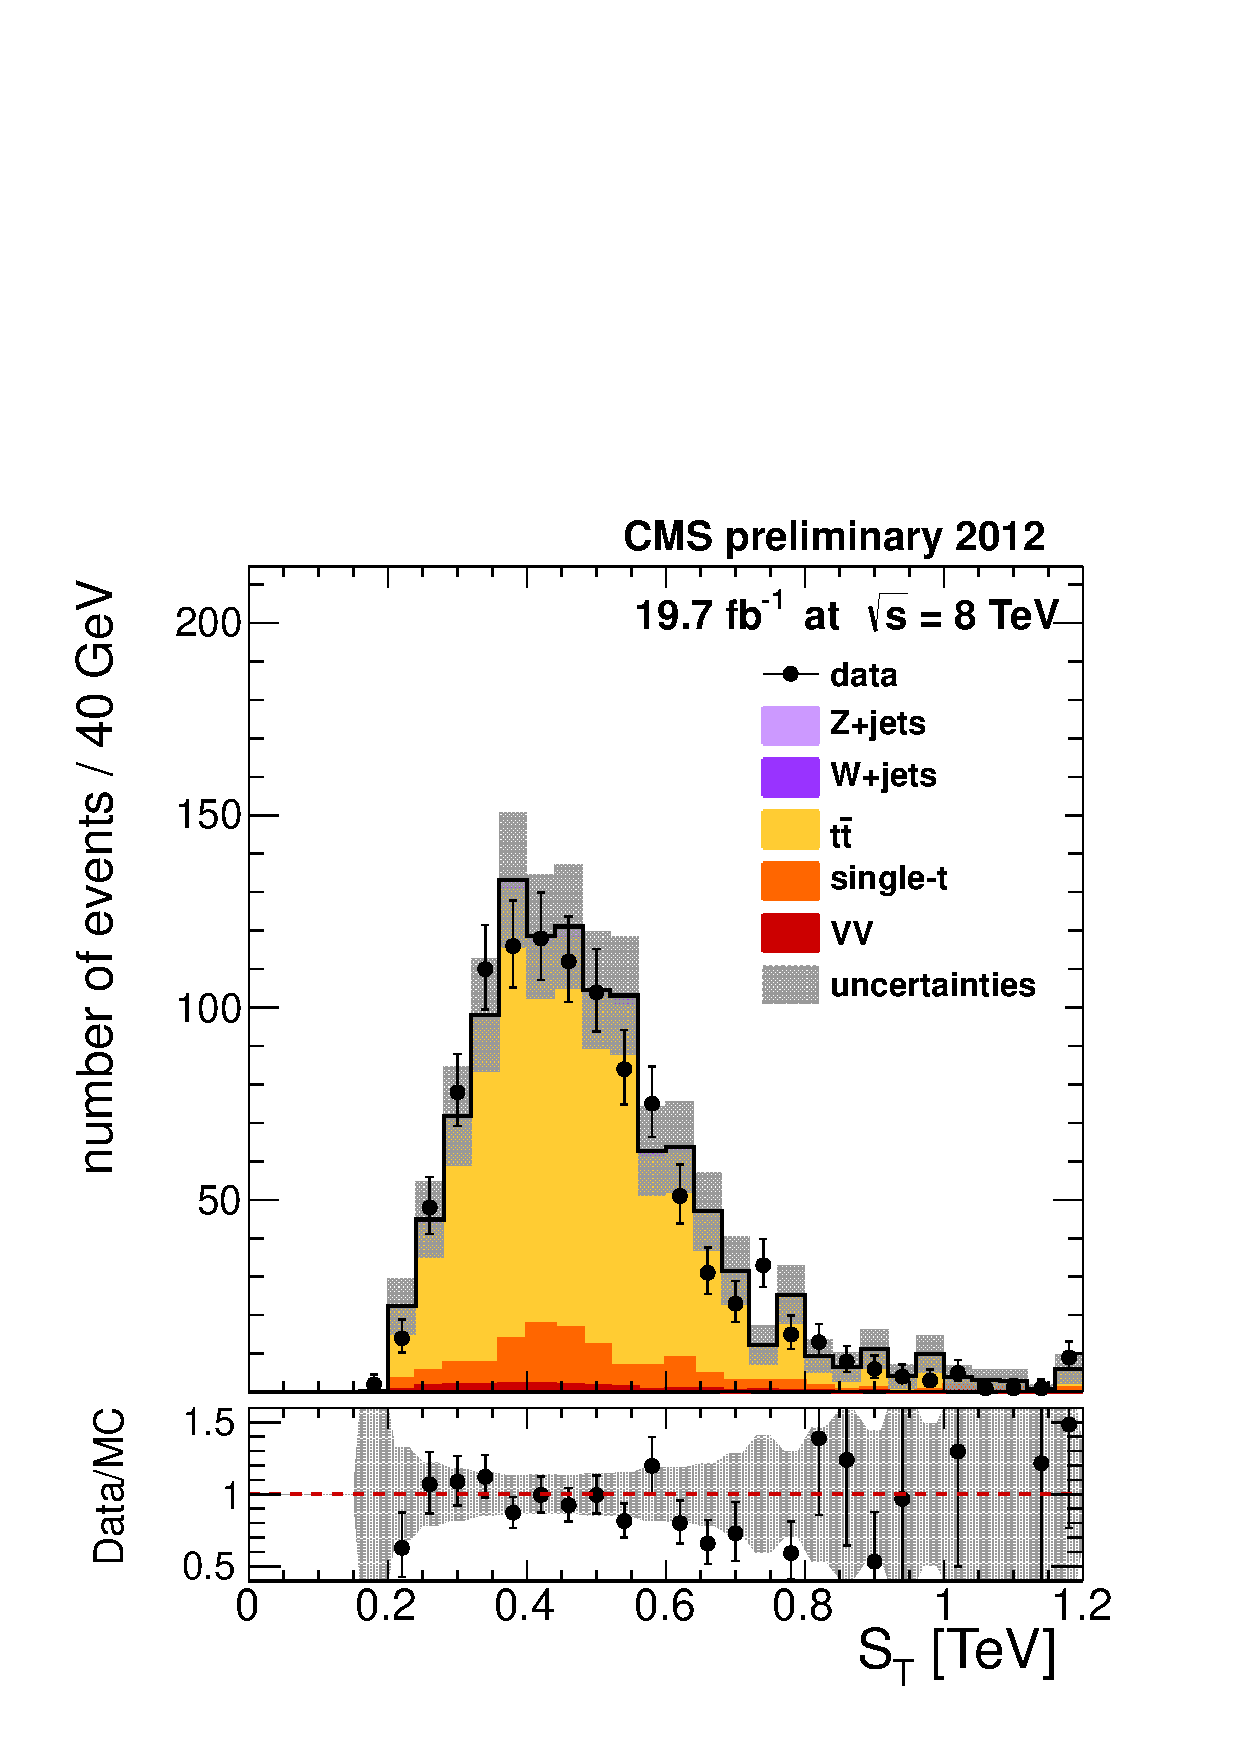
\includegraphics[width=0.49\textwidth]{figures/bkgEstim/STbjetFinalEMu.pdf}
    \caption{The \ST distribution in the $\emu$ control region after the leptoquark final selection. The uncertainty band reflects the statistical uncertainty in the simulated backgrounds.}
    \label{fig:ttCC}
  \end{center}
\end{figure}


The \ttbar yields in the \emu control region, $N_{\emu}$, and in the signal regions, $N_{\ltau}$, are defined in Eqs. \eqref{eq:Nemu} and \eqref{eq:Nltau}. Throughout this section, the convention $\ell = \Pe, \mu$ will be used.
\begin{alignat}{2}
\label{eq:Nemu}
  N_{\emu} &= \sigma \mathcal{L} &&\times \left(\Ee \Emu \varepsilon^{\text{sel}}_{\emu} \rho^{\text{sel}}_{\emu} \right)  \nonumber \\
           &                     &&\times 2 \left[\vphantom{\Btm} \Aem\Be\Bm + \Amte\Bm\Bte \right. \\
           &                     &&+ \left. \Aetm\Be\Btm  + \Atetm\Bte\Btm \right],  \nonumber \\
 N_{\ltau} &= \sigma \mathcal{L} &&\times \left(\El \Eth \varepsilon^{\text{sel}}_{\ltau} \rho^{\text{sel}}_{\ltau} \right) \nonumber \\
           &                     &&\times 2 \left[\Alth\Bl\Bth + \Atlth\Btl\Bth \right].  \label{eq:Nltau}
\end{alignat}
Here, $\sigma$ is the \ttbar production cross section; $\mathcal{L}$ is the integrated luminosity; $\varepsilon_{x}^{\text{ID}}$ is the selection efficiency for the identification and isolation of a lepton $x$ in the simulation; $\varepsilon^{\text{sel}}_{i}$ is the analysis selection efficiency in the simulation, including the jet multiplicity cut, the b-tagging requirement, and so forth, for the channel $i$; and $\rho^{\text{sel}}_{i}$ is the simulation to data scale factor associated with the selection efficiency for the channel $i$. The branching fractions $\mathcal{B}$ of the \W boson decay for each leptonic decay channel are labeled as follows:
\begin{align}
\mathcal{B}(\W \rightarrow \ell \nu_{\ell}) &= \Bl, \\
\mathcal{B}(\W \rightarrow \tau\nu_{\tau} \rightarrow \ell \nu_{\tau} \nu_{\ell}) &= \Btl, \\
\mathcal{B}(\W \rightarrow \tau\nu_{\tau} \rightarrow \text{hadrons} + \nu_{\tau}) &= \Bth.
\end{align}
Similarly, the acceptance for a process creating one lepton $\ell$ and one lepton $\ell^{\prime}$ is called $\mathcal{A}_{\ell\ell^{\prime}}$. The acceptances are computed using the MC simulation of the \ttbar process and are defined for each leptonic decay channel:
\begin{equation}
  \mathcal{A} = \frac{N_{\text{sel}}(\ell\ell^{\prime})}{N_{\text{gen}}(\ell\ell^{\prime})}.
\end{equation}
$N_{\text{gen}}(\ell\ell^{\prime})$ is the number of generated events containing two leptons $\ell$ and $\ell^{\prime}$, and $N_{\text{sel}}(\ell\ell^{\prime})$ is the number of those generated events that are selected when kinematic requirements are imposed. The requirements used are the \pt and $\eta$ cuts used for the selection of the primary electrons, muons, and hadronic taus in the signal region. The acceptances for each decay channel are listed in Table \ref{tab:TTAcc}.

\begin{table}
  \begin{center}
    \begin{tabular}{|l|r|c|l|r|}
      \cline{1-2}\cline{4-5}
      channel & \multicolumn{1}{c|}{$\mathcal{A}$ (\%)} && channel & \multicolumn{1}{c|}{$\mathcal{A}$ (\%)} \\
      \cline{1-2}\cline{4-5}
      $\Pe\tauh$ & $23.6\pm0.3$ && $\mu\tauh$ & $23.7\pm0.3$ \\
      $\tau_{\Pe}\tauh$ & $10.4\pm0.5$ && $\tau_{\mu}\tauh$ & $10.5\pm0.4$ \\
      $\Pe\tau_{\mu}$ & $13.9\pm0.4$ && $\mu\tau_{\Pe}$ & $12.3\pm0.4$ \\
      $\Pe\mu$ & $41.6\pm0.3$ && $\tau_{\Pe}\tau_{\mu}$ & $3.4\pm0.5$ \\
      \cline{1-2}\cline{4-5}
    \end{tabular}
    \caption{Acceptances (in \%) for the \ttbar process in each leptonic decay channel of the \W boson produced by the top quark decays. Variations in the acceptances are mostly due to differences in the \pt distributions for each type of lepton.}
    \label{tab:TTAcc}
  \end{center}
\end{table}

Equations \eqref{eq:Nltau} and \eqref{eq:Nemu} can be combined to eliminate $\sigma\mathcal{L}$, which produces a formula to extrapolate the \ttbar yield from the \emu control region to the \ltau signal region:
\begin{align}
\label{eq:ttbartot}
N_{\ltau} &= N_{\emu} \times \frac{\El\Eth}{\Ee\Emu} \times \frac{\varepsilon^{\text{sel}}_{\ltau}\rho^{\text{sel}}_{\ltau}}{\varepsilon^{\text{sel}}_{\emu}\rho^{\text{sel}}_{\emu}} \nonumber \\
&\times \frac{\Alth\Bl\Bth + \Atlth\Btl\Bth}{\Aem\Be\Bm + \Amte\Bm\Bte + \Aetm\Be\Btm + \Atetm\Bte\Btm}.
\end{align}
$N_{\emu}$ is the yield from the \emu control region in the observed data, with the residual non-\ttbar background subtracted. The yield in the signal region $N_{\ltau}$ is extrapolated from $N_{\emu}$ via multiplication by selection and identification efficiencies, data/MC scale factors, acceptances, and branching fractions.

The selection efficiencies $\varepsilon$ and the data/MC scale factors $\rho$ are derived from several different sources. The standard efficiencies for the lepton identification algorithms are computed in \Z events. However, differences in topology between \ttbar and \Z events make these values inappropriate for the \ttbar background estimation. The identification efficiencies are therefore calculated using simulated \ttbar events. The reconstructed leptons in these events are required to be matched with genuine leptons at the generator level, and the results are listed in Table \ref{tab:ttlepeff}. The standard efficiencies for the HLT criteria are used. The standard data/MC scale factors for the lepton identification, HLT efficiency, and b-tagging are also used. The difference in performance between the observed data and the MC simulation is assumed to be due to inherent properties of the simulation without any dependence on the type of event.

\begin{table}
  \begin{center}
    \begin{tabular}{|c|c|c|}
      \hline
      lepton & $\varepsilon$ from \ttbar events (\%) & $\rho$ from \Z events \\
      \hline\hline
      \Pe     & $77.3 \pm 0.1$ & $1.011 \pm 0.001$ \\
      $\mu$   & $81.3 \pm 0.1$ & $0.995 \pm 0.001$ \\
      $\tauh$ & $35.5 \pm 4.9$ & $1.000\vphantom{{}\pm0.001}$ \\
      \hline
    \end{tabular}
    \caption{Lepton identification efficiencies $\varepsilon$ measured in simulated \ttbar events and associated scale factors $\rho$ measured in \Z events.}
    \label{tab:ttlepeff}
  \end{center}
\end{table}

The analysis selection efficiencies are calculated using the \ttbar simulation. The efficiencies are computed for each selection requirement, including: vertex matching between the two leptons, opposite charge between the two leptons, additional lepton veto, $N_{\text{jets}}\geq2$, $N_{\text{b-jets}}\geq1$, and $\pt(\tauh)>50\GeV$. The final selection cuts $\MassTJ>250\GeV$ for the leptoquark search and $N_{\text{jets}}\geq5$ for the top squark search are also considered. In order to compute the data/MC scale factors in a \ttbar enriched sample, the order of the selection cuts is altered. First, the jet multiplicity requirement is applied: $N_{\text{jets}}\geq2$ for the leptoquark search or $N_{\text{jets}}\geq5$ for the top squark search. Next, the b-tagging requirement is applied, and then the \MassTJ cut is applied for the leptoquark search. The other selection requirements are applied subsequently.

The overall data/MC scale factors associated with the vertex matching, opposite charge, lepton veto, and final hadronic tau \pt cut are computed in the control region defined by requiring events with two b-jets and $\MassTJ<120\GeV$. The separate control region with $120\GeV < \MassTJ < 250\GeV$ is used to check that the scale factors do not depend on the value of the $\MassTJ$ cuts. Due to the lack of a pure \ttbar control region to estimate the data/MC scale factor at the level of the jet multiplicity requirement, no scale factor is applied and an additional systematic uncertainty is assigned. For similar reasons, no scale factor is applied for the \MassTJ cut. The results of these selection efficiency and scale factor calculations are listed in Table \ref{tab:tteff}.

\afterpage{
\begin{landscape}
\begin{table}
  \begin{center}
    \begin{tabular}{|l|r|c|r|c|r|c|}
      \hline
      \multirow{2}{*}{Selection} & \multicolumn{2}{c|}{$\etau$ channel} & \multicolumn{2}{c|}{$\mutau$ channel} & \multicolumn{2}{c|}{$\emu$ channel} \\
      \cline{2-7}
      & \multicolumn{1}{c|}{$\varepsilon$ (\%)} & $\rho$ & \multicolumn{1}{c|}{$\varepsilon$ (\%)} & $\rho$ & \multicolumn{1}{c|}{$\varepsilon$ (\%)} & $\rho$ \\
      \hline \hline
      $\varepsilon_{\ell}\varepsilon_{\ell^{\prime}}$ & $27.4\pm0.1$ & $1.011\pm0.001$ & $28.9\pm0.1$ & $0.995\pm0.001$ & $62.8\pm0.1$ & $1.006\pm0.001$ \\
      $\varepsilon_{\text{HLT}}$ & $91.4\pm0.1$ & $-$ & $89.2\pm0.1$ & $-$ & $89.2\pm0.1$ & $-$ \\ 
      \hline
      & \multicolumn{6}{c|}{Leptoquark search} \\ 
      \hline
      $\varepsilon_{\text{jet}}$ & $76.1\pm0.5$ & $-$ & $74.1\pm0.5$ & $-$ & $79.5\pm0.2$ & $-$ \\
      $\varepsilon_{\text{b-tag}}$ & $94.2\pm0.3$ & $-$ & $92.7\pm0.4$ & $-$ & $94.0\pm0.1$ & $-$ \\
      $\varepsilon_{\text{vtx},~\text{OS},~\ell~\text{veto},~\pt(\tauh)}$ & $38.2\pm1.5$ & $0.987\pm0.042$ & $38.2\pm1.6$ & $0.947\pm0.038$ & $60.5\pm1.0$ & $1.002\pm0.020$ \\
      $\varepsilon_{\text{mass}}$ & $6.8\pm0.6$ & $-$ & $5.3\pm0.6$ & $-$ & $7.1\pm0.1$ & $-$ \\ 
      \hline
      & \multicolumn{6}{c|}{Top squark search} \\ 
      \hline
      $\varepsilon_{\text{jet}}$ & $3.7\pm0.2$ & $-$ & $2.8\pm0.2$ & $-$ & $4.2\pm0.2$ & $-$ \\
      $\varepsilon_{\text{b-tag}}$ & $98.3\pm0.3$ & $-$ & $99.0\pm0.3$ & $-$ & $98.0\pm0.1$ & $-$ \\
      $\varepsilon_{\text{vtx},~\text{OS},~\ell~\text{veto},~\pt(\tauh)}$ & $51.7\pm2.0$ & $0.987\pm0.042$ & $45.9\pm2.1$ & $0.947\pm0.038$ & $66.7\pm2.0$ & $1.002\pm0.020$ \\
      \hline
    \end{tabular}
    \caption{The relative selection efficiencies (in \%) and data/MC scale factors $\rho$ for the \ttbar process in each channel \etau, \mutau, and \emu. The total selection efficiency is the product of all the relative selection efficiencies for a given search.}
    \label{tab:tteff}
  \end{center}
\end{table}
\end{landscape}
}

The systematic uncertainty assigned to the jet multiplicity requirement is defined as the difference between data and simulation in the efficiency of the requirement. This difference is calculated in a control region consisting of 95\% \ttbar events, which is selected by requiring both \W bosons in each event to decay to muons. Additional requirements are applied to reduce the contamination from non-\ttbar processes: $\met > 50\GeV$, $20\GeV < M_{\mu\mu} < 70\GeV$ or $M_{\mu\mu} > 120\GeV$. The data/MC differences in the efficiency of the jet multiplicity requirements are found to be 1\% for $N_{\text{jets}}\geq2$ in the leptoquark search and 3\% for $N_{\text{jets}}\geq5$ in the top squark search. These differences are propagated through the \ttbar estimation method as systematic uncertainties.

The systematic uncertainty assigned to the \MassTJ requirement is calculated from two sources. The first source is the relative difference between the efficiencies in data and simulation in the $\ttbar \rightarrow \mu\mu$ control sample, which is found to be 6\%. The second source is the difference between the efficiencies obtained in data in the $\emu$ channel with and without the residual non-\ttbar background. This difference is also found to be 6\%. The two sources are taken to be independent, so they are added in quadrature to produce a total uncertainty of 8.5\%.

To describe the calculation of the total systematic uncertainty from the propagation of the uncertainty in the acceptances, efficiencies, and scale factors, it is instructive to assign shorthand notation to the factors in Eq. \eqref{eq:ttbartot}:
\begin{equation}
\label{eq:ttbartot2}
N_{\ltau} = N_{\emu} \times R_{\text{ID}} \times R_{\text{sel}} \times R_{\mathcal{A}\mathcal{B}}.
\end{equation}
As indicated by comparing Eq. \eqref{eq:ttbartot} and Eq. \eqref{eq:ttbartot2}, $R_{\text{ID}}$ is the ratio of the identification efficiencies, $R_{\text{sel}}$ is the ratio of the selection efficiencies and scale factors, and $R_{\mathcal{A}\mathcal{B}}$ is the ratio of the acceptances and branching fractions. Equation \eqref{eq:dsyst} shows a simplified version of the propagation of the uncertainties from these three ratio factors:
\begin{equation}
\label{eq:dsyst}
\delta_{\text{syst}} = \sqrt{ (\delta_{\text{ID}} \times R_{\text{sel}} \times R_{\mathcal{A}\mathcal{B}})^2 + (R_{\text{ID}} \times \delta_{\text{sel}} \times R_{\mathcal{A}\mathcal{B}})^2 + (R_{\text{ID}} \times R_{\text{sel}} \times \delta_{\mathcal{A}\mathcal{B}})^2}.
\end{equation}
The uncertainty in the ratio $R_x$ is written as $\delta_x$. In the particular case of $\delta_{\text{sel}}$, the uncertainty value is modified by the additional uncertainties assigned to the $N_{\text{jets}}$ and \MassTJ cuts, as discussed above:
\begin{equation}
\delta_{\text{sel}} \rightarrow \sqrt{ \delta_{\text{sel}}^2 + (R_{\text{sel}} \times U_{N_{\text{jets}}})^2 + (R_{\text{sel}} \times U_{\MassTJ})^2}.
\end{equation}
$U_x$ is the additional uncertainty associated with the cut $x$. In the top squark search, the uncertainty associated with the \MassTJ cut is not included, as that cut is not applied.

Using Eq. \ref{eq:ttbartot}, the extrapolated yield of the \ttbar irreducible background is computed for each \ltau channel. The results are summarized in Table \ref{tab:ttYieldsLQ} for the leptoquark search and in Table \ref{tab:ttYieldsLQD} for the top squark search. This estimation method is applied to a simulated \emu sample as a cross-check, and the results agree within one standard deviation when compared to the expectation from the direct simulation of the irreducible \ttbar contributions to the \ltau channels. The extrapolation from observed data is also in agreement with both the expectation from the direct \ttbar \ltau simulation and the extrapolation from the \emu simulation. For each \ltau channels, the \ttbar \ST distribution is estimated from the exclusive $\ttbar \rightarrow b\ell\nu b\ell\nu$ MC simulation.

\begin{table}[hbt]
  \begin{center}
    \begin{tabular}{|l|c|c|c|}
	  \multicolumn{4}{c}{Leptoquark search} \\
      \hline
      \multirow{3}{*}{} & \multicolumn{3}{c|}{$\emu$ channel} \\
      \cline{2-4}
      & \ttbar MC & data & data $-$ residual MC \\
      \cline{2-4}
      & $966.71\pm27.3$ & $1065 ({}\pm 32.6)$ & $920.0\pm8.3 \pm 32.6$  \\
      \hline\hline
      \multirow{2}{*}{} & \multicolumn{3}{c|}{$\ltau$ channel} \\
      \hline
      channel & \ttbar MC (genuine \tauh) & \ttbar MC extrap. & data extrap. \\
      \hline
      $\etau$         & $94.4\pm8.3$ & $94.0\pm2.7\pm14.9$ & $98.7\pm3.6\pm17.7$ \\ %2.6*1.3
      $\mutau$       & $72.8\pm8.5$ & $72.2\pm2.0\pm12.6$ & $64.2\pm2.3\pm12.4$ \\ %2.9*1.3
      \hline
    \end{tabular}
    \caption{The estimated \ttbar irreducible yields after the leptoquark final selection, from: direct simulation, extrapolation from the $\emu$ simulation, and extrapolation from the observed $\emu$ data. In the extrapolated results, the first uncertainty value corresponds to the statistical uncertainty in the simulation and observed data, while the second uncertainty value corresponds to the propagation of the uncertainties in the acceptances, efficiencies and scale factors. }
    \label{tab:ttYieldsLQ}
  \end{center}
\end{table}

\begin{table}[hbt]
  \begin{center}
    \begin{tabular}{|l|c|c|c|}
      \multicolumn{4}{c}{Top squark search} \\
      \hline
      \multirow{3}{*}{} & \multicolumn{3}{c|}{$\emu$ channel} \\
      \cline{2-4}
      & \ttbar MC & data & data $-$ residual MC \\
      \cline{2-4}
      & $823.9\pm26.3$ & $733 ({}\pm 27.1)$ & $700.0\pm7.2 \pm 27.1$ \\
      \hline\hline
      \multirow{2}{*}{} & \multicolumn{3}{c|}{$\ltau$ channel} \\
      \hline
      channel & \ttbar MC (genuine \tauh) & \ttbar MC extrap. & data extrap. \\
      \hline
      $\etau$         & $80.4\pm7.5$ & $81.7\pm2.6\pm12.5$ & $76.6\pm3.1\pm13.3$ \\
      $\mutau$       & $57.9\pm6.4$ & $65.8\pm2.1\pm10.3$ & $52.2\pm2.1\pm9.3$ \\
      \hline
    \end{tabular}
    \caption{The estimated \ttbar irreducible yields after the top squark final selection, from: direct simulation, extrapolation from the $\emu$ simulation, and extrapolation from the observed $\emu$ data. In the extrapolated results, the first uncertainty value corresponds to the statistical uncertainty in the simulation and observed data, while the second uncertainty value corresponds to the propagation of the uncertainties in the acceptances, efficiencies and scale factors. }
    \label{tab:ttYieldsLQD}
  \end{center}
\end{table}

This estimation of the \ttbar irreducible background estimation does not account for events with jets or leptons misidentified as hadronic taus, but does include events with jets or photons misidentified as electrons or muons. The yield from events in which an electron or a muon is identified as a hadronic tau is estimated from the simulation and added to the yield of the \ttbar irreducible background. This contribution is estimated to be $6.9\pm 2.1$ ($2.5\pm 1.3$) for the \etau (\mutau) channel in the leptoquark search and $11.7\pm 2.7$ ($2.8 \pm 1.3$) for the \etau (\mutau) channel in the top squark search. The small statistical uncertainty from this contribution is neglected when adding it to the \ttbar irreducible yield. The estimation of the background from events with jets misidentified as hadronic taus will be discussed in the next section.